\chapter{\ifproject%
\ifenglish Project Structure and Methodology\else โครงสร้างและขั้นตอนการทำงาน\fi
\else%
\ifenglish Project Structure\else โครงสร้างของโครงงาน\fi
\fi
}

ในบทนี้จะกล่าวถึงภาพรวมของ BEVA ที่จะสร้างว่ามีการใช้งานอย่างไร 
การทำงานของ Dialogflow พร้อมทั้งการจัดการ database และการออกแบบฝั่ง Web server และ ฝั่ง client

\makeatletter

% \renewcommand\section{\@startsection {section}{1}{\z@}%
%                                    {13.5ex \@plus -1ex \@minus -.2ex}%
%                                    {2.3ex \@plus.2ex}%
%                                    {\normalfont\large\bfseries}}

\makeatother
%\vspace{2ex}
% \titleformat{\section}{\normalfont\bfseries}{\thesection}{1em}{}
% \titlespacing*{\section}{0pt}{10ex}{0pt}

\section{โครงสร้าง}
  \begin{figure}[hbt!]
    \begin{center}
    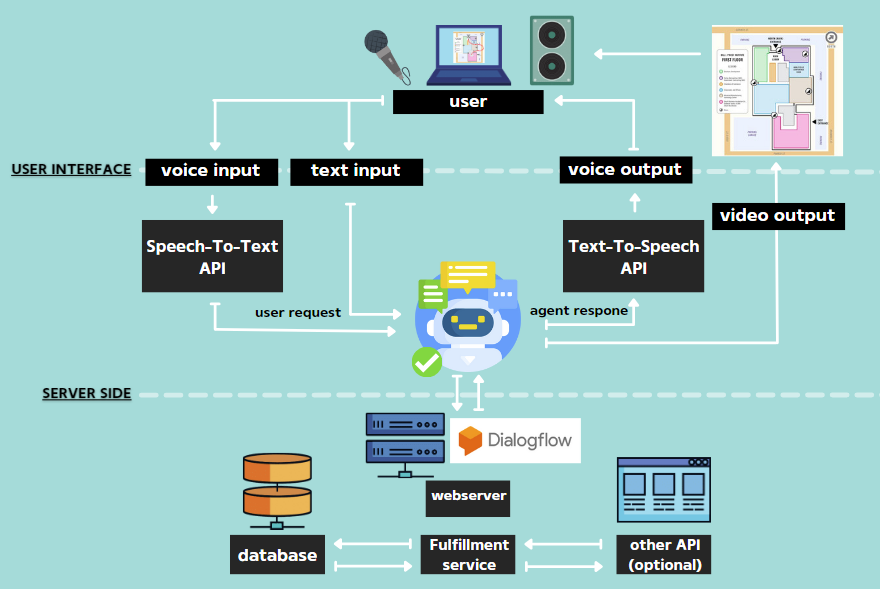
\includegraphics[width=\textwidth,keepaspectratio]{pic/overview.png}
    \end{center}
    \caption{Project Overview}
    \label{fig:overview}
  \end{figure}
โปรเจคนี้ทำการพัฒนาแชทบอทผ่าน Dialogflow ที่เชื่อมต่อกับ Web application และทำการเชื่อมต่อเขียน
โปรแกรมโดยใช้ NodeJS ดึงข้อมูลจาก Database โดยชนิดของ Database ที่ใช้เป็นแบบ NoSQL ซึ่งเมื่อผู้ใช้
ถามคำถามผ่านทางการพูดใส่ไมค์ที่อยู่บริเวณอาคาร ตัว Web จะส่ง user request Google STT ก่อนเพื่อแปลง
เสียงที่ได้รับมาให้กลายเป็นข้อความและตอบกลับมาที่เว็บหลังจากได้ตัวข้อความแล้วก็จะส่ง user request ไปยัง
Dialogflow ซึ่งคำถามที่ส่งมานั้นจะถูกแยกออกเป็น 3 กรณีนั่นคือ

\begin{enumerate}
  \item ไม่ต้องการข้อมูลจาก database หรือ API: คำตอบจะถูกส่งคืนกลับไปเป็น agent response
  ของ Dialogflow
  \item ต้องการข้อมูลจาก database: Dialogflow จะทำการส่ง API ไปที่ webhook จากนั้นจะทำการ
  ดึงข้อมูลจาก database แล้วส่งกลับไปยัง Dialogflow ในรูปแบบของ JSON เพื่อให้ Dialogflow ส่ง
  คำตอบให้ผู้ใช้งานต่อไป
  \item ต้องการข้อมูลจาก API: Dialogflow จะทำการส่ง API ไปที่ webhook จากนั้นจะทำการข้อมูล
  ซึ่ง API จะตอบกลับมาในรูปของ JSON ให้กับ Dialogflow และให้ Dialogflow ส่งคำตอบให้ผู้ใช้งานอีกที่
\end{enumerate}

\section{รูปแบบการเก็บข้อมูลใน Cloud Firestore}
รูปแบบในการเก็บข้อมูลที่เลือกใช้จะเป็นแบบ NoSQL บน Cloud Firestore~\cite{fs-doc} ซึ่งเราได้วางโครงสร้างไว้ดังนี้ 
\begin{figure}[hbt!]
  \begin{center}
  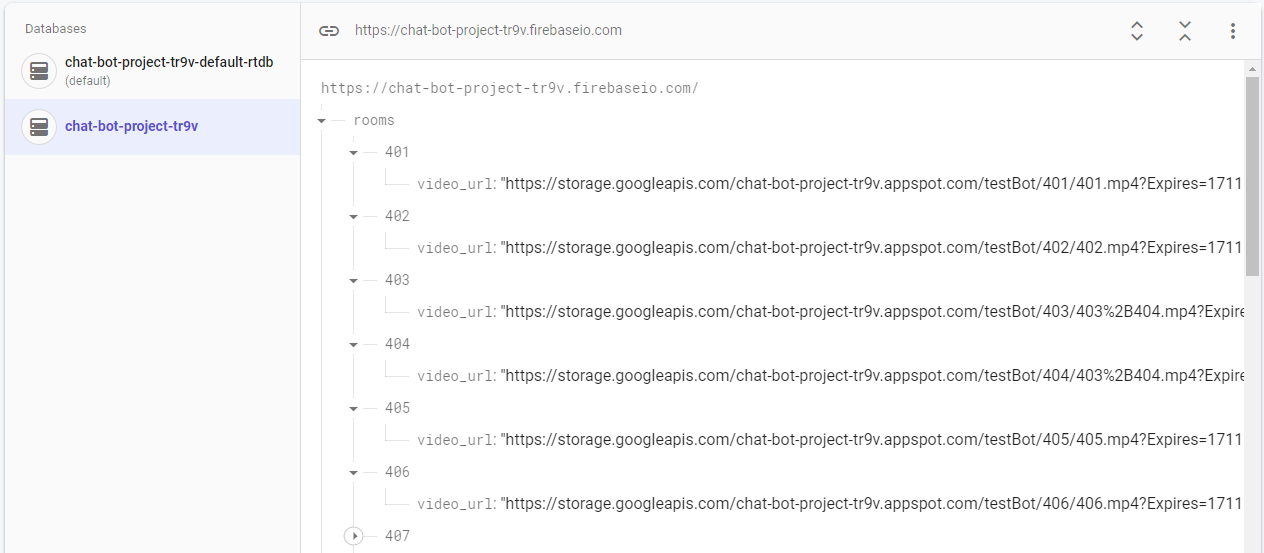
\includegraphics[width=\textwidth,keepaspectratio]{pic/database_mapPath.png}
  \end{center}
  \caption{การเก็บข้อมูลที่อยู่ของไฟล์ video แผนที่สำหรับแต่ละห้อง}
  \label{fig:db_mapPath}
\end{figure}

\section{รูปแบบการเก็บข้อมูลใน Cloud Storage}
รูปแบบในการเก็บข้อมูลที่อยู่บน Cloud Storage จะมีลักษณะเหมือนกับ Google Drive เราสามารถอัพโหลดไฟล์ขึ้นไปฝากไว้บน Cloud
ได้โดยบนนี้เราจะเก็บไฟล์ video ที่แสดงเส้นทางไปยังห้องต่างๆในแต่ละชั้นดังนี้
\begin{figure}[hbt!]
  \begin{center}
  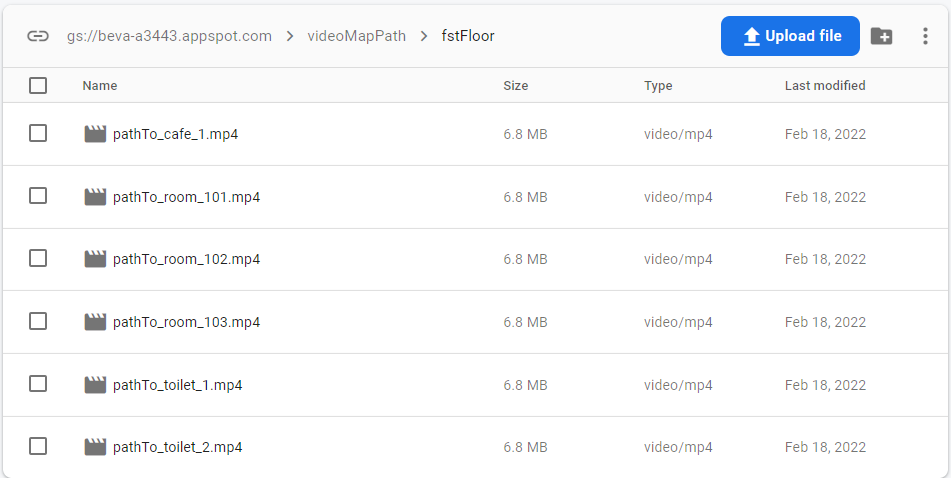
\includegraphics[width=\textwidth,keepaspectratio]{pic/db_storage.png}
  \end{center}
  \caption{การเก็บข้อมูลไฟล์ video แผนที่สำหรับแต่ละห้อง}
  \label{fig:db_storage}
\end{figure}

\begin{figure}[hbt!]
  \begin{center}
  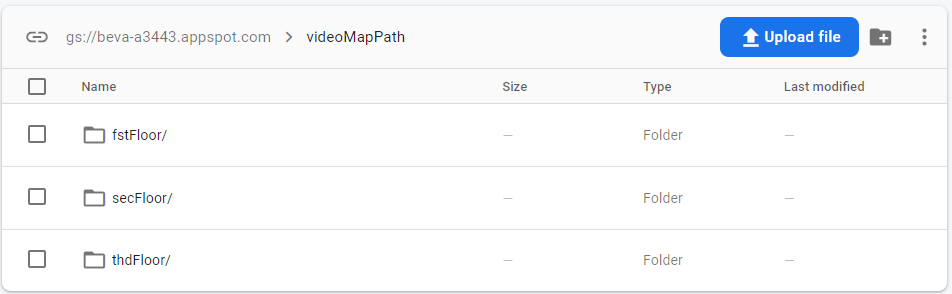
\includegraphics[width=\textwidth,keepaspectratio]{pic/db_storage_floorFolder.png}
  \end{center}
  \caption{folder สำหรับเก็บ video ของแผนที่สำหรับแต่ละห้อง}
  \label{fig:db_storage_floorFolder}
\end{figure}
\section{รูปแบบการเก็บข้อมูลใน Cloud Storage}
\section{รูปแบบการเก็บข้อมูลใน Cloud Storage}